\documentclass{article}
\usepackage{tenor2015}
\usepackage{times}
\usepackage{ifpdf}
\usepackage[english]{babel}
\usepackage{cite}
\usepackage{microtype}

\usepackage[scaled=0.95]{inconsolata}
\usepackage{verbatim}

\usepackage{listings}
\lstset{
basicstyle=\scriptsize\ttfamily,
breakatwhitespace=false,
breaklines=false,	
escapeinside={(*@}{@*)},
keywordstyle=\bfseries,
language=Python,
showspaces=false,
showstringspaces=false,
showtabs=false,
xleftmargin=2mm
}

\def\papertitle{Abjad:
An open-source software system for Formalized Score Control}
\def\firstauthor{Trevor Ba\v{c}a}
\def\secondauthor{Josiah Wolf Oberholtzer}
\def\thirdauthor{Jeffrey Trevi\~{n}o}
\def\fourthauthor{V\'{i}ctor Ad\'{a}n}

\newif\ifpdf
\ifx\pdfoutput\relax
\else
   \ifcase\pdfoutput
      \pdffalse
   \else
      \pdftrue
\fi

\ifpdf % compiling with pdflatex
  \usepackage[pdftex,
    pdftitle={\papertitle},
    pdfauthor={\firstauthor, \secondauthor, \thirdauthor, \fourthauthor},
    bookmarksnumbered, % use section numbers with bookmarks
    pdfstartview=XYZ % start with zoom=100% instead of full screen;
                     % especially useful if working with a big screen :-)
   ]{hyperref}
  %\pdfcompresslevel=9

  \usepackage[pdftex]{graphicx}
  % declare the path(s) where your graphic files are and their extensions so
  %you won't have to specify these with every instance of \includegraphics
  \graphicspath{{./figures/}}
  \DeclareGraphicsExtensions{.pdf,.jpeg,.png}

  \usepackage[figure,table]{hypcap}

\else % compiling with latex
  \usepackage[dvips,
    bookmarksnumbered, % use section numbers with bookmarks
    pdfstartview=XYZ % start with zoom=100% instead of full screen
  ]{hyperref}  % hyperrefs are active in the pdf file after conversion
  \usepackage[dvips]{epsfig,graphicx}
  \graphicspath{{./figures/}}
  \DeclareGraphicsExtensions{.eps}
  \usepackage[figure,table]{hypcap}
\fi

\hypersetup{
    colorlinks,
    citecolor=black,
    filecolor=black,
    linkcolor=black,
    urlcolor=black
}

%\title{\papertitle}
\title{Abjad: \\
an open-source software system \\
for Formalized Score Control}

\fourauthors
  {\firstauthor} {Harvard University \\
    {\tt \href{mailto:trevor.baca@gmail.com}
        {trevor.baca@gmail.com}}}
  {\secondauthor} {Harvard University \\
    {\tt \href{mailto:josiah.oberholtzer@gmail.com}
        {josiah.oberholtzer@gmail.com}}}
  {\thirdauthor} {Carleton College \\
    {\tt \href{mailto:jeffrey.trevino@gmail.com}
        {jeffrey.trevino@gmail.com}}}
  {\fourthauthor} {
    {\tt \href{mailto:vctradn@gmail.com}
        {vctradn@gmail.com}}}

\begin{document}

\capstartfalse
\maketitle
\capstarttrue

\begin{abstract}
The Abjad API for Formalized Score Control extends the Python programming
language with an open-source, object-oriented software system that enables
composers to build scores through the encoded aggregation of elemental notation
objects. A summary of widely used notation systems' intended uses motivates a
discussion of system design priorities via examples of system use.
\end{abstract}
\section{Introduction} \label{sec:introduction}

Abjad\footnote{www.projectabjad.org} is an open-source software
system designed to help composers build scores in an iterative and incremental
way.  Abjad is implemented in the Python\footnote{www.python.org} programming
language as an object-oriented collection of packages, classes
and functions. Composers can visualize their work as publication-quality
notation at all stages of the compositional process using Abjad's interface to
the LilyPond\footnote{www.lilypond.org} music notation package. The first
versions of Abjad were implemented in 1997 and the project website is now
visited thousands of times each month. This paper details some of the most
important principles guiding the development of Abjad and illustrates these with examples of the system in use. The priorities outlined
here arise in answer to domain-specific questions of music modeling (What are
the fundamental elements of music notation? Which elements of music notation
should be modeled hierarchically?) as well as in consideration of the ways in which best practices taken
from software engineering can apply to the development of a music software
system (How can programming concepts iteration,
aggregation and encapsulation help composers as they work?).
A background taxonomy motivates a discussion of design priorities via examples
of system use.

\section{A Taxonomy} \label{sec:taxonomy}

Many software systems implement models of music but few of these
implement a model of notation.\footnote{Computational models of music might
entail the representation of higher-level musical entities apparent in the acts
of listening and analysis but absent in the symbols of notation themselves, as
determined to be creatively exigent. Programming researchers and musical
artists have modeled many such extrasymbolic musical entities, such as
large-scale form and transition \cite{polansky1991morphological,
uno1994temporal, dobrian1995algorithmic, abrams1999higher,
Yoo1983}, texture \cite{Horenstein:2004kx}, contrapuntal relationships
\cite{Boenn:2009oq, Bell:1995ij, farbood2001analysis, Cope:2002fv, Laurson:2005dz, Polansky:2011fu, Ebcioglu:1980kl}, harmonic
tension and resolution \cite{Melo2003, Wiggins1999, Foster:1995qa}, melody \cite{Hornel:1993mi, Smith:1992pi}, meter
\cite{Hamanaka:2005ff}, rhythm \cite{Nauert2007, Degazio:1996lh, Collins:2003bs}, timbre \cite{Xenakis:1991fu, Creasey:1996ye, Osaka2004}, temperament \cite{Seymour:2007qo, Graf:2006il} and ornamentation \cite{Ariza:2003zt, Chico-Topfer:1998jl}. This work
overlaps fruitfully with analysis tasks, and models of listening and cognition
can enable novel methods of high-level musical structures and transformations,
like dramatic direction, tension, and transition between sections
\cite{Collins2009}.} Music software systems that model notation can be
classified according to their generative tasks.\footnote{Software production
exists as an organizationally designed feedback loop between production values
and implementation \cite{Derniame:1999fk}, and it is possible to understand a
system by understanding the purpose for which it was initially designed. This
purpose can be termed a software system's generative task. In the analysis of
systems created for use by artists, this priority yields a dilemma instantly,
as analyses that explain a system's affordances with reference to intended
purpose must contend with the creative use of technology by artists: a system's
intended uses might have little or nothing in common with the way in which the
artist finally uses the technology. For this reason, the notion of generative
task is best understood as an explanation for a system's affordances, with the
caveat that a user can nonetheless work against those affordances to use the
system in novel ways. Generative tasks --- informed by the cultural milieu of
software development, economic constraints of software production, and the
aesthetic proclivities of artists participating in development processes ---
constrain software features to enable a limited subset of possible
representations and user interactions.

While composers working traditionally may allow intuition to substitute for
formally defined principles, a computer demands the composer to think formally
about music \cite{Xenakis:1992rq}. Keeping in mind generative task as an
analytical framework, it is broadly useful to bifurcate a  notation
system's development into the modeling of composition, on the one
hand, and the modeling of musical notation, on the other. All systems model
both, to greater or lesser degrees, often engaging in the ambiguous or implicit
modeling of composition while focusing more ostensibly on a model of
notation, or focusing on the abstract modeling of music without a considered
link to a model of notation. Due to the intimate link between notation and
musical ideas, it is impossible for a system that models notation to avoid at
least implicitly modeling musical and compositional ideas, and a computational
model of music and composition is an inevitable component of every
notation system, even when it exists as an unspoken set of technological
constraints. Generative task explains a given system's balance between
computational models of composition and notation by assuming a link
between intended use and system development.}

Many notation systems --- such as Finale, Sibelius, SCORE \cite{Smith:1972mw},
Igor, Berlioz, Lilypond \cite{Nienhuys:2003ve}, GUIDO \cite{Hoos:1998bd}
NoteAbility \cite{hamel1noteability}, FOMUS \cite{Psenicka2006,Psenicka2009} and Nightingale --- exist to help people engrave and format music documents; because these systems provide functions
that operate on notational elements (i.e., transposition, spacing and
playback), hidden models of common practice music notation must underly all of
these systems, and each system's interface constrains and directs the ways in
which users interact with this underlying model of notation. These systems
enable users to engrave and format music without exposing any particular
underlying model of composition, and without requiring, or even inviting the
user to computationally model composition. Such systems might go so far as to
enable scripting, as in the case of Sibelius's ManuScript \cite{Technology:qc}
scripting language or Lilypond's embedded Scheme code; although these systems
enable the automation of notational elements, it remains difficult to model
compositional processes and relationships.

Other systems provide environments specifically for the modeling of
higher-level processes and relationships. OpenMusic \cite{Assayag:1999sw}, PWGL
\cite{Laurson:2009qf} and BACH \cite{agostini2013real} supply an interface to
a model of common practice notation, as well as a set of non-common-practice visual interfaces that enables the user to model composition, in the context of a stand-alone application and with the aid of the above notation editors for final engraving and layout via intermediate file formats. Similarly purposed systems extend text-based programming languages rather than existing as stand-alone applications, such as HMSL's extension of Forth \cite{Polansky:1990fk}, JMSL's extension of Java \cite{didkovsky2001java} and Common Music's extension of Lisp \cite{taube1991common}. Other composition modeling systems, such as athenaCL \cite{Ariza2005} and PILE/AC Toolbox \cite{Berg1979} provide a visual interface for the creation of compositional structures without providing a model of common practice notation.

Some composers make scores with software systems that provide neither a model
of notation nor a model of composition. Graphic layout programs, such as
AutoCAD and Adobe Illustrator, have been designed broadly for the placement and
design of graphic elements. While scripting enables automation, composers must
model both notation and composition from scratch, and the symbolic scope of
potential automations described in the course of modeling ensures that
composers spend as much time addressing elemental typographical concerns (e.g.,
accidental collisions) as would be spent modeling compositional processes and
relationships.

Many models of musical notation have been designed for purposes of
corpus-based computational musicology. Formats such as DARM, SMDL,
HumDrum and MuseData model notation with the generative task of searching
through a large amount of data \cite{Selfridge-Field:1997ud}. Commercial
notation software developers attempted to establish a data interchange standard
for optical score recognition (NIFF) \cite{niff1995niff}. Since its release in
2004, MusicXML has become a valid interchange format for over 160 applications
and maintains a relatively application-agnostic status, as it was designed with
the generative task of acting as an interchange format between variously tasked
systems \cite{Good:2001if}.\footnote{An attempt to more
comprehensively survey the history of object-oriented notation systems for
composition, in the context of the broader history of object-oriented
programming, lies beyond the scope of this paper but has recently been
undertaken elsewhere\cite{trevino2013compositional}.}

\section{Abjad basics} \label{sec:example}

Abjad is not a stand-alone application. Nor is Abjad a programming language.
Abjad instead adds a computational model of music notation to the Python
programming language. By designing Abjad as an extension to one of the most
widely-used programming languages in the world, we hope to make a considerable
collection of programming best practices available to composers in a
straightforward way. Abjad is implemented as a Python package;\footnote{See the
Python Package Index for extensions to Python for purposes as diverse as
creative writing and aeronautical engineering. The Python Package Index
contains 54,306 packages at the time or writing and is available at
\textit{https://pypi.python.org}.}\footnote{Designing Abjad as an extension to Python makes hundreds of print and Web Python
resources relevant to composers working in Abjad. The global
community of developers working in Python also becomes available to composers,
and vice versa.}\footnote{Abjad is an importable Python library. It can be used in whole or in part as a
component of any Python-compatible system. For example, Abjad supports IPython Notebook, a web-based interactive computational environment combining code execution, text, mathematics, plots
and rich media into a single document. Notational output from Abjad can be
transparently captured and embedded into an IPython Notebook that has
loaded Abjad's IPython Notebook extension. See \textit{http://ipython.org/notebook.html}.}
composers work with Abjad exactly the same
way developers work with all the other packages available for the language. In
the most common case this means opening a file, writing code and saving the
file:

\begin{comment}
<abjad>[strip_prompt=true]
from abjad import *

def make_nested_tuplet(
    tuplet_duration,
    outer_tuplet_proportions,
    inner_tuplet_subdivision_count,
    ):
    outer_tuplet = Tuplet.from_duration_and_ratio(
        tuplet_duration, outer_tuplet_proportions)
    inner_tuplet_proportions = \
        inner_tuplet_subdivision_count * [1]
    last_leaf = outer_tuplet.select_leaves()[-1]
    inspector = inspect_(last_leaf)
    right_logical_tie = inspector.get_logical_tie()
    right_logical_tie.to_tuplet(inner_tuplet_proportions)
    return outer_tuplet
</abjad>
\end{comment}

%%% ABJADBOOK START %%%
\begin{lstlisting}
from abjad import *

def make_nested_tuplet(
    tuplet_duration,
    outer_tuplet_proportions,
    inner_tuplet_subdivision_count,
    ):
    outer_tuplet = Tuplet.from_duration_and_ratio(
        tuplet_duration, outer_tuplet_proportions)
    inner_tuplet_proportions = \
        inner_tuplet_subdivision_count * [1]
    last_leaf = outer_tuplet.select_leaves()[-1]
    inspector = inspect_(last_leaf)
    right_logical_tie = inspector.get_logical_tie()
    right_logical_tie.to_tuplet(inner_tuplet_proportions)
    return outer_tuplet
\end{lstlisting}
%%% ABJADBOOK END %%%

\noindent The contents of the file can then be used in other Python files or in
an interactive session:

\begin{comment}
<abjad>
rhythmic_staff = Staff(context_name='RhythmicStaff')
tuplet = make_nested_tuplet((7, 8), (3, -1, 2), 3)
rhythmic_staff.append(tuplet)
show(rhythmic_staff)
</abjad>
\end{comment}

%%% ABJADBOOK START %%%
\begin{lstlisting}
>>> rhythmic_staff = Staff(context_name='RhythmicStaff')
>>> tuplet = make_nested_tuplet((7, 8), (3, -1, 2), 3)
>>> rhythmic_staff.append(tuplet)
>>> show(rhythmic_staff)
\end{lstlisting}
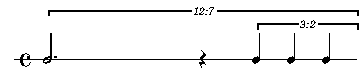
\includegraphics{assets/lilypond-a8fcfb8f401a81a10afeb01a4f9f03ab.pdf}
%%% ABJADBOOK END %%%

\noindent This paper demonstrates most examples in Python's interactive console
because the console helps distinguish input from output;\footnote{Lines
preceded by the \texttt{>>>} prompt are passed to Python for interpretation;
any output generated by the line of code appears immediately after. The example
above creates a tuplet with the tuplet-making function defined earlier and
calls Abjad's top-level \texttt{show()} function to generate a PDF of the
result.} however, composers work with Abjad primarily by typing
notationally-enabled Python code into a collection of interrelated files and
managing those files as a project grows to encompass the composition of an
entire score.\footnote{The importance Abjad attaches to composers' ability to
notate the objects they work with during composition should be underscored
before proceeding to more detailed examples. Abjad reflects this priority in
its illustration protocol, which conventionalizes the way developers equip
Abjad classes with notation output and the way composers notate objects during
composition. Abjad's top-level \texttt{show()} function, included in most of
the examples in this article, implements the composer-facing part of this
protocol and provides a unified way to notate any object in the system. A
collection of \texttt{\_\_illustrate\_\_()} methods implement the
developer-facing part of this protocol and define the way any given class
should produce notation. Under the most common pattern, Abjad transforms an
object into LilyPond input code and then calls LilyPond to render the input as
a PDF.}

\begin{comment}
\footnote{Python describes common informal
interfaces to working with objects as \emph{protocols}. Important protocols
include the \emph{iterator protocol} for iterating over the contents of a
container-like object, the \emph{sequence protocol} for getting items and
length from a container-like object and the \emph{mutable container protocol}
for mutating the contents of a container-like object.}
\end{comment}

\begin{comment}
\footnote{Abjad's illustration protocol decouples illustration logic
from the other functions of a class. An important consequence of this is that
developers can illustrate classes with LaTeX or GraphViz or any collection of
applications, whether or not LilyPond is included in the tool chain. We find
LilyPond superior for a formalized score control system like Abjad for many
reasons, ranging from LilyPond's powerful model of rhythmic timekeeping to the
high quality of LilyPond output. But should the need arise to replace LilyPond
with a different typesetting engine, the composer-facing  interface provided by
\texttt{show()} will remain the same. The priority is that composers be able to
illustrate compositional objects. LilyPond simply happens to be the best
resource available to achieve our goals.}
\end{comment}

\section{The Abjad object model} \label{sec:object-model}

Abjad models musical notation with \emph{components}, \emph{spanners} and
\emph{indicators}. Every notational element in Abjad belongs to one of these
three families. Abjad models notes, rests and chords as classes that can be
added into the container-like elements of music notation, such as tuplets,
measures, voices, staves and complete scores.\footnote{Abjad uses the term
`leaf' to refer generally to notes, rests, and chords. This term, borrowed from
graph theory, reflects the fact that notes, rests and chords cannot contain
other elements of music notation.} Spanners model notational constructs that
cross different levels of hierarchy in the score tree, such as beams, slurs and
glissandi. Indicators model objects attached to a single component, such as
articulations, dynamics and time signatures.\footnote{Abjad indicators are
scoped. Indicator scoping models how all notes in a voice can be marked
\emph{forte} until another note is marked \emph{piano}. We have generalized the
scoping behavior of indicators, allowing composers to annotate score structures
by attaching arbitrary non-notating objects like dictionaries or custom classes
to any component.} Composers arrange components hierarchically into a score
tree with spanners and indicators attached to components in the tree.

\section{Bottom-up construction} \label{sec:bottom-up}

Abjad lets composers build scores from the bottom up. When working bottom-up,
composers create individual notes, rests and chords to be grouped into tuplets,
measures and voices that may then be included in even high-level containers,
such as staves and scores.\footnote{Unlike many notation packages, Abjad does
not require composers to structure music into measures. Abjad's tuple, voice,
staff, and score container components can hold leaves (notes, rests and chords)
directly.}\footnote{Notes, rests and chords may be initialized with pitches named according to either American or European conventions, with the pitch numbers of American pitch-class theory or from combinations of Abjad pitch and duration objects.} Abjad implements this style of component aggregation via a
collection of methods which append, extend or insert into container-like
components as though they were lists:\footnote{Abjad's container interface
derives from Python's mutable sequence protocol, which specifies an interface
to list-like objects.}

\begin{comment}
<abjad>
outer_tuplet_one = Tuplet((2, 3), "d''16 f'8.")
inner_tuplet = Tuplet((4, 5), "cs''16 e'16 d'2")
outer_tuplet_one.append(inner_tuplet)
outer_tuplet_two = Tuplet((4, 5))
outer_tuplet_two.extend("d'8 r16 c'16 bf'16")
tuplets = [outer_tuplet_one, outer_tuplet_two]
upper_staff = Staff(tuplets, name='Upper Staff')
note_one = Note(10, (3, 16))
upper_staff.append(note_one)
note_two = Note(NamedPitch("fs'"), Duration(1, 16))
upper_staff.append(note_two)
lower_staff = Staff(name='Lower Staff')
lower_staff.extend("c8 r8 b8 r8 gf8 r4 cs8")
staff_group = StaffGroup()
staff_group.extend([upper_staff, lower_staff])
score = Score([staff_group])
show(score)
</abjad>
\end{comment}

%%% ABJADBOOK START %%%
\begin{lstlisting}
>>> outer_tuplet_one = Tuplet((2, 3), "d''16 f'8.")
>>> inner_tuplet = Tuplet((4, 5), "cs''16 e'16 d'2")
>>> outer_tuplet_one.append(inner_tuplet)
>>> outer_tuplet_two = Tuplet((4, 5))
>>> outer_tuplet_two.extend("d'8 r16 c'16 bf'16")
>>> tuplets = [outer_tuplet_one, outer_tuplet_two]
>>> upper_staff = Staff(tuplets, name='Upper Staff')
>>> note_one = Note(10, (3, 16))
>>> upper_staff.append(note_one)
>>> note_two = Note(NamedPitch("fs'"), Duration(1, 16))
>>> upper_staff.append(note_two)
>>> lower_staff = Staff(name='Lower Staff')
>>> lower_staff.extend("c8 r8 b8 r8 gf8 r4 cs8")
>>> staff_group = StaffGroup()
>>> staff_group.extend([upper_staff, lower_staff])
>>> score = Score([staff_group])
>>> show(score)
\end{lstlisting}
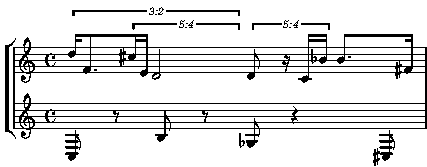
\includegraphics{assets/lilypond-45865c9ff19c72c1c9f7a6f4234e8546.pdf}
%%% ABJADBOOK END %%%

\noindent Ties, slurs and other spanners attach to score components via Abjad's
top-level \texttt{attach()} function. The same is true for articulations, clefs
and other indicators:

\begin{comment}
<abjad>
upper_leaves = upper_staff.select_leaves()
lower_leaves = lower_staff.select_leaves()
attach(Tie(), upper_leaves[4:6])
attach(Tie(), upper_leaves[-3:-1])
attach(Slur(), upper_leaves[:2])
attach(Slur(), upper_leaves[2:6])
attach(Slur(), upper_leaves[7:])
attach(Articulation('accent'), upper_leaves[0])
attach(Articulation('accent'), upper_leaves[2])
attach(Articulation('accent'), upper_leaves[7])
attach(Clef('bass'), lower_leaves[0])
show(score)
</abjad>
\end{comment}

%%% ABJADBOOK START %%%
\begin{lstlisting}
>>> upper_leaves = upper_staff.select_leaves()
>>> lower_leaves = lower_staff.select_leaves()
>>> attach(Tie(), upper_leaves[4:6])
>>> attach(Tie(), upper_leaves[-3:-1])
>>> attach(Slur(), upper_leaves[:2])
>>> attach(Slur(), upper_leaves[2:6])
>>> attach(Slur(), upper_leaves[7:])
>>> attach(Articulation('accent'), upper_leaves[0])
>>> attach(Articulation('accent'), upper_leaves[2])
>>> attach(Articulation('accent'), upper_leaves[7])
>>> attach(Clef('bass'), lower_leaves[0])
>>> show(score)
\end{lstlisting}
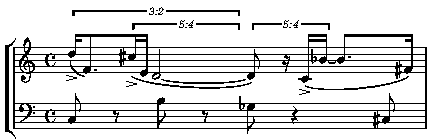
\includegraphics{assets/lilypond-b8f044cb7178ea31797238c629d3f54c.pdf}
%%% ABJADBOOK END %%%

\noindent When does it make sense for composers to work with Abjad in the
bottom-up way outlined here? Instantiating components by hand in the way shown
above resembles notating by hand and composers may choose to work bottom-up
when doing the equivalent of sketching in computer code: when making the first
versions of a figure or gesture, when trying out combinations of small bits of
notation or when inserting one or two items at a time into a larger structure.
For some composers this may be a regular or even predominant way of working.
Other composers may notice patterns in their own compositional process when
they work bottom-up and may find ways to formalize these patterns into classes
or functions that generalize their work; the next section describes some ways
composers might do this.

%The ability to combine score components one by one into ever-larger aggregates
%gives composers fine-grained control over their compositional structures;
%however, as composers notice bottom-up work patterns, they may desire to
%formalize these patterns into component-generating factory functions. In this
%way, bottom-up work may proceed in ongoing dialogue with top-down strategies
%of score construction.

\section{Top-down construction} \label{sec:top-down}

What are the objects of music composition? For most composers, individual
notes, rests and chords constitute  only the necessary means to achieve some
larger, musically interesting result. For this reason, a model of composition
needs to describe groups of symbols on the page: notes taken in sequence to
constitute a figure, gesture or melody; chords taken in sequence as a
progression; attack points arranged in time as the scaffolding of some larger
texture. These entities, and the others like them, might result from a flash of
compositional intuition that then requires detailed attention and elaboration.

Abjad invites composers to implement factories as a way of generalizing and
encapsulating parts of one's own compositional process. In this way, composers
can extend the system as they work to implement their own models of
composition. Abjad also provides a variety of factory functions and factory
classes that exemplify this way of working. These range from simple
note-generating functions, like \texttt{make\_notes()}, which combine sequences
of pitches and rhythms to generate patterned selections of notes and rests, to
more complexly-configured maker classes for creating nuanced rhythmic patterns
or entire scores.

As an example, consider the \texttt{rhythmmakertools} package included with
Abjad. The classes provided in this package are factory classes which, once
configured, can be called like functions to inscribe rhythms into a series of
beats or other time divisions. The example below integrates configurable
patterns of durations, tupletting and silences:

\begin{comment}
<abjad>
burnish_specifier = rhythmmakertools.BurnishSpecifier(
    left_classes=(Rest, Note),
    left_counts=(1,),
    )
talea = rhythmmakertools.Talea(
    counts=(1, 2, 3),
    denominator=16,
    )
tie_specifier = rhythmmakertools.TieSpecifier(
    tie_across_divisions=True,
    )
rhythm_maker = rhythmmakertools.TaleaRhythmMaker(
    burnish_specifier=burnish_specifier,
    extra_counts_per_division=(0, 1, 1),
    talea=talea,
    tie_specifier=tie_specifier,
    )
divisions = [(3, 8), (5, 16), (1, 4), (3, 16)]
show(rhythm_maker, divisions=divisions)
</abjad>
\end{comment}

%%% ABJADBOOK START %%%
\begin{lstlisting}
>>> burnish_specifier = rhythmmakertools.BurnishSpecifier(
...     left_classes=(Rest, Note),
...     left_counts=(1,),
...     )
>>> talea = rhythmmakertools.Talea(
...     counts=(1, 2, 3),
...     denominator=16,
...     )
>>> tie_specifier = rhythmmakertools.TieSpecifier(
...     tie_across_divisions=True,
...     )
>>> rhythm_maker = rhythmmakertools.TaleaRhythmMaker(
...     burnish_specifier=burnish_specifier,
...     extra_counts_per_division=(0, 1, 1),
...     talea=talea,
...     tie_specifier=tie_specifier,
...     )
>>> divisions = [(3, 8), (5, 16), (1, 4), (3, 16)]
>>> show(rhythm_maker, divisions=divisions)
\end{lstlisting}
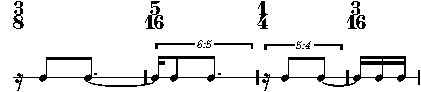
\includegraphics{assets/lilypond-c238b5fdf445554d95cebd52911b461e.pdf}
%%% ABJADBOOK END %%%

\noindent Once instantiated, factory classes like this can be used over and
over again with different input:

\begin{comment}
<abjad>
rhythmic_score = Score()
for i in range(8):
    selections = rhythm_maker(divisions, seeds=i)
    measure = Measure((9, 8), selections)
    staff = Staff(context_name='RhythmicStaff')
    staff.append(measure)
    rhythmic_score.append(staff)
    divisions = sequencetools.rotate_sequence(
        divisions, 1)

show(rhythmic_score)
</abjad>
\end{comment}

%%% ABJADBOOK START %%%
\begin{lstlisting}
>>> rhythmic_score = Score()
>>> for i in range(8):
...     selections = rhythm_maker(divisions, seeds=i)
...     measure = Measure((9, 8), selections)
...     staff = Staff(context_name='RhythmicStaff')
...     staff.append(measure)
...     rhythmic_score.append(staff)
...     divisions = sequencetools.rotate_sequence(
...         divisions, 1)
...
>>> show(rhythmic_score)
\end{lstlisting}
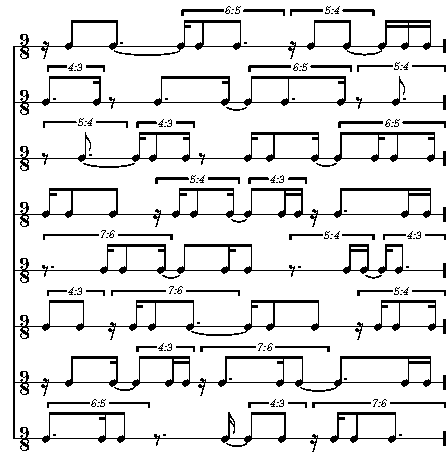
\includegraphics{assets/lilypond-89acf493fafea6ee83e3032bbed09718.pdf}
%%% ABJADBOOK END %%%

\begin{comment}
\section{Input flexibility} \label{sec:input-flexibility}

Input flexibility allows composers to create compositional objects in whatever
way aligns with their conception of music and with the task at hand
\cite{Kay:1996vn}. Abjad's score components can be created in a variety of
ways. Notes and chords can be instantiated parametrically by specifying pitch
and rhythm information numerically. These elements can also be created via
explicit \texttt{Pitch} and \texttt{Duration} objects. Containers, such as
tuplets and measures, can be instantiated parametrically by specifying explicit
lists of components to be inserted as children. Abjad also allows many score
objects to be created via strings parseable in one of the various
micro-languages we have implemented. Score components created via string input
can be potentially much more complex than those created parametrically, because
Abjad's microlanguage parsers have the ability to attach spanners and
indicators to both the created components and their children (if the created
components are containers). Parametric instantiation gives composers powerful
procedural control over score structure while string instantiation provides
concisely specified expression. The score construction examples above
demonstrates both of these techniques.
\end{comment}

\section{Selecting Objects in the Score} \label{sec:selection-flexibility}

Abjad allows composers to select and operate on collections of
objects in a score. Composers can select objects in several
ways: by name, numeric indices or iteration.
A single operation, such as transposing pitches or attaching articulations,
can then be mapped onto the entirety of a selection.

\noindent Consider the two-staff score created earlier. Because both staves were given
explicit names, the upper staff can be selected by name:

\begin{comment}
<abjad>
upper_staff = score['Upper Staff']
show(upper_staff)
</abjad>
\end{comment}

%%% ABJADBOOK START %%%
\begin{lstlisting}
>>> upper_staff = score['Upper Staff']
>>> show(upper_staff)
\end{lstlisting}
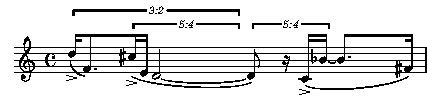
\includegraphics{assets/lilypond-dcce2b5927dd4f606034c3efcde7da2e.pdf}
%%% ABJADBOOK END %%%

\noindent Using numeric indices, the lower staff can be selected by indexing
the second child of the first child of the score:

\begin{comment}
<abjad>
lower_staff = score[0][1]
show(lower_staff)
</abjad>
\end{comment}

%%% ABJADBOOK START %%%
\begin{lstlisting}
>>> lower_staff = score[0][1]
>>> show(lower_staff)
\end{lstlisting}
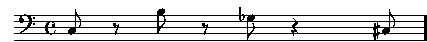
\includegraphics{assets/lilypond-fa746e527d218a814e36af2f46d314bb.pdf}
%%% ABJADBOOK END %%%

\noindent The top-level \texttt{iterate()} function exposes Abjad's score
iteration interface. This interface provides a collection of methods for
iterating the components in a score in different ways. For example, all
notes can be selected from a single staff:

\begin{comment}
<abjad>
for note in iterate(lower_staff).by_class(Note):
    attach(Articulation('staccato'), note)

show(score)
</abjad>
\end{comment}

%%% ABJADBOOK START %%%
\begin{lstlisting}
>>> for note in iterate(lower_staff).by_class(Note):
...     attach(Articulation('staccato'), note)
...
>>> show(score)
\end{lstlisting}
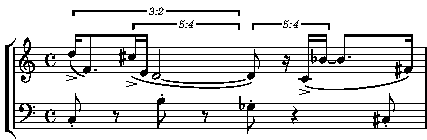
\includegraphics{assets/lilypond-b7a01ad584c3c470c0bbff20fbc76741.pdf}
%%% ABJADBOOK END %%%

\noindent Groups of tied notes can be selected from an entire
score:\footnote{Abjad uses the term \emph{logical tie} to refer to a selection
of one or more leaf components which represent all of the components tied
together by zero or more ties; a single note, untied, is considered a
\emph{trivial} logical tie.}


\begin{comment}
<abjad>
for logical_tie in iterate(score).by_logical_tie():
    if 1 < len(logical_tie):
        attach(Fermata(), logical_tie.tail)
        for note in logical_tie:
            override(note).note_head.style = 'cross'

show(score)
</abjad>
\end{comment}

%%% ABJADBOOK START %%%
\begin{lstlisting}
>>> for logical_tie in iterate(score).by_logical_tie():
...     if 1 < len(logical_tie):
...         attach(Fermata(), logical_tie.tail)
...         for note in logical_tie:
...             override(note).note_head.style = 'cross'
...
>>> show(score)
\end{lstlisting}
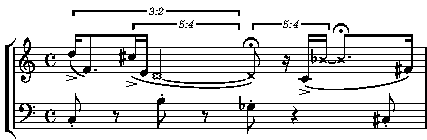
\includegraphics{assets/lilypond-a692b35a07435259861a4299267be394.pdf}
%%% ABJADBOOK END %%%

\begin{figure*}
    \centering
    \makebox[\textwidth]{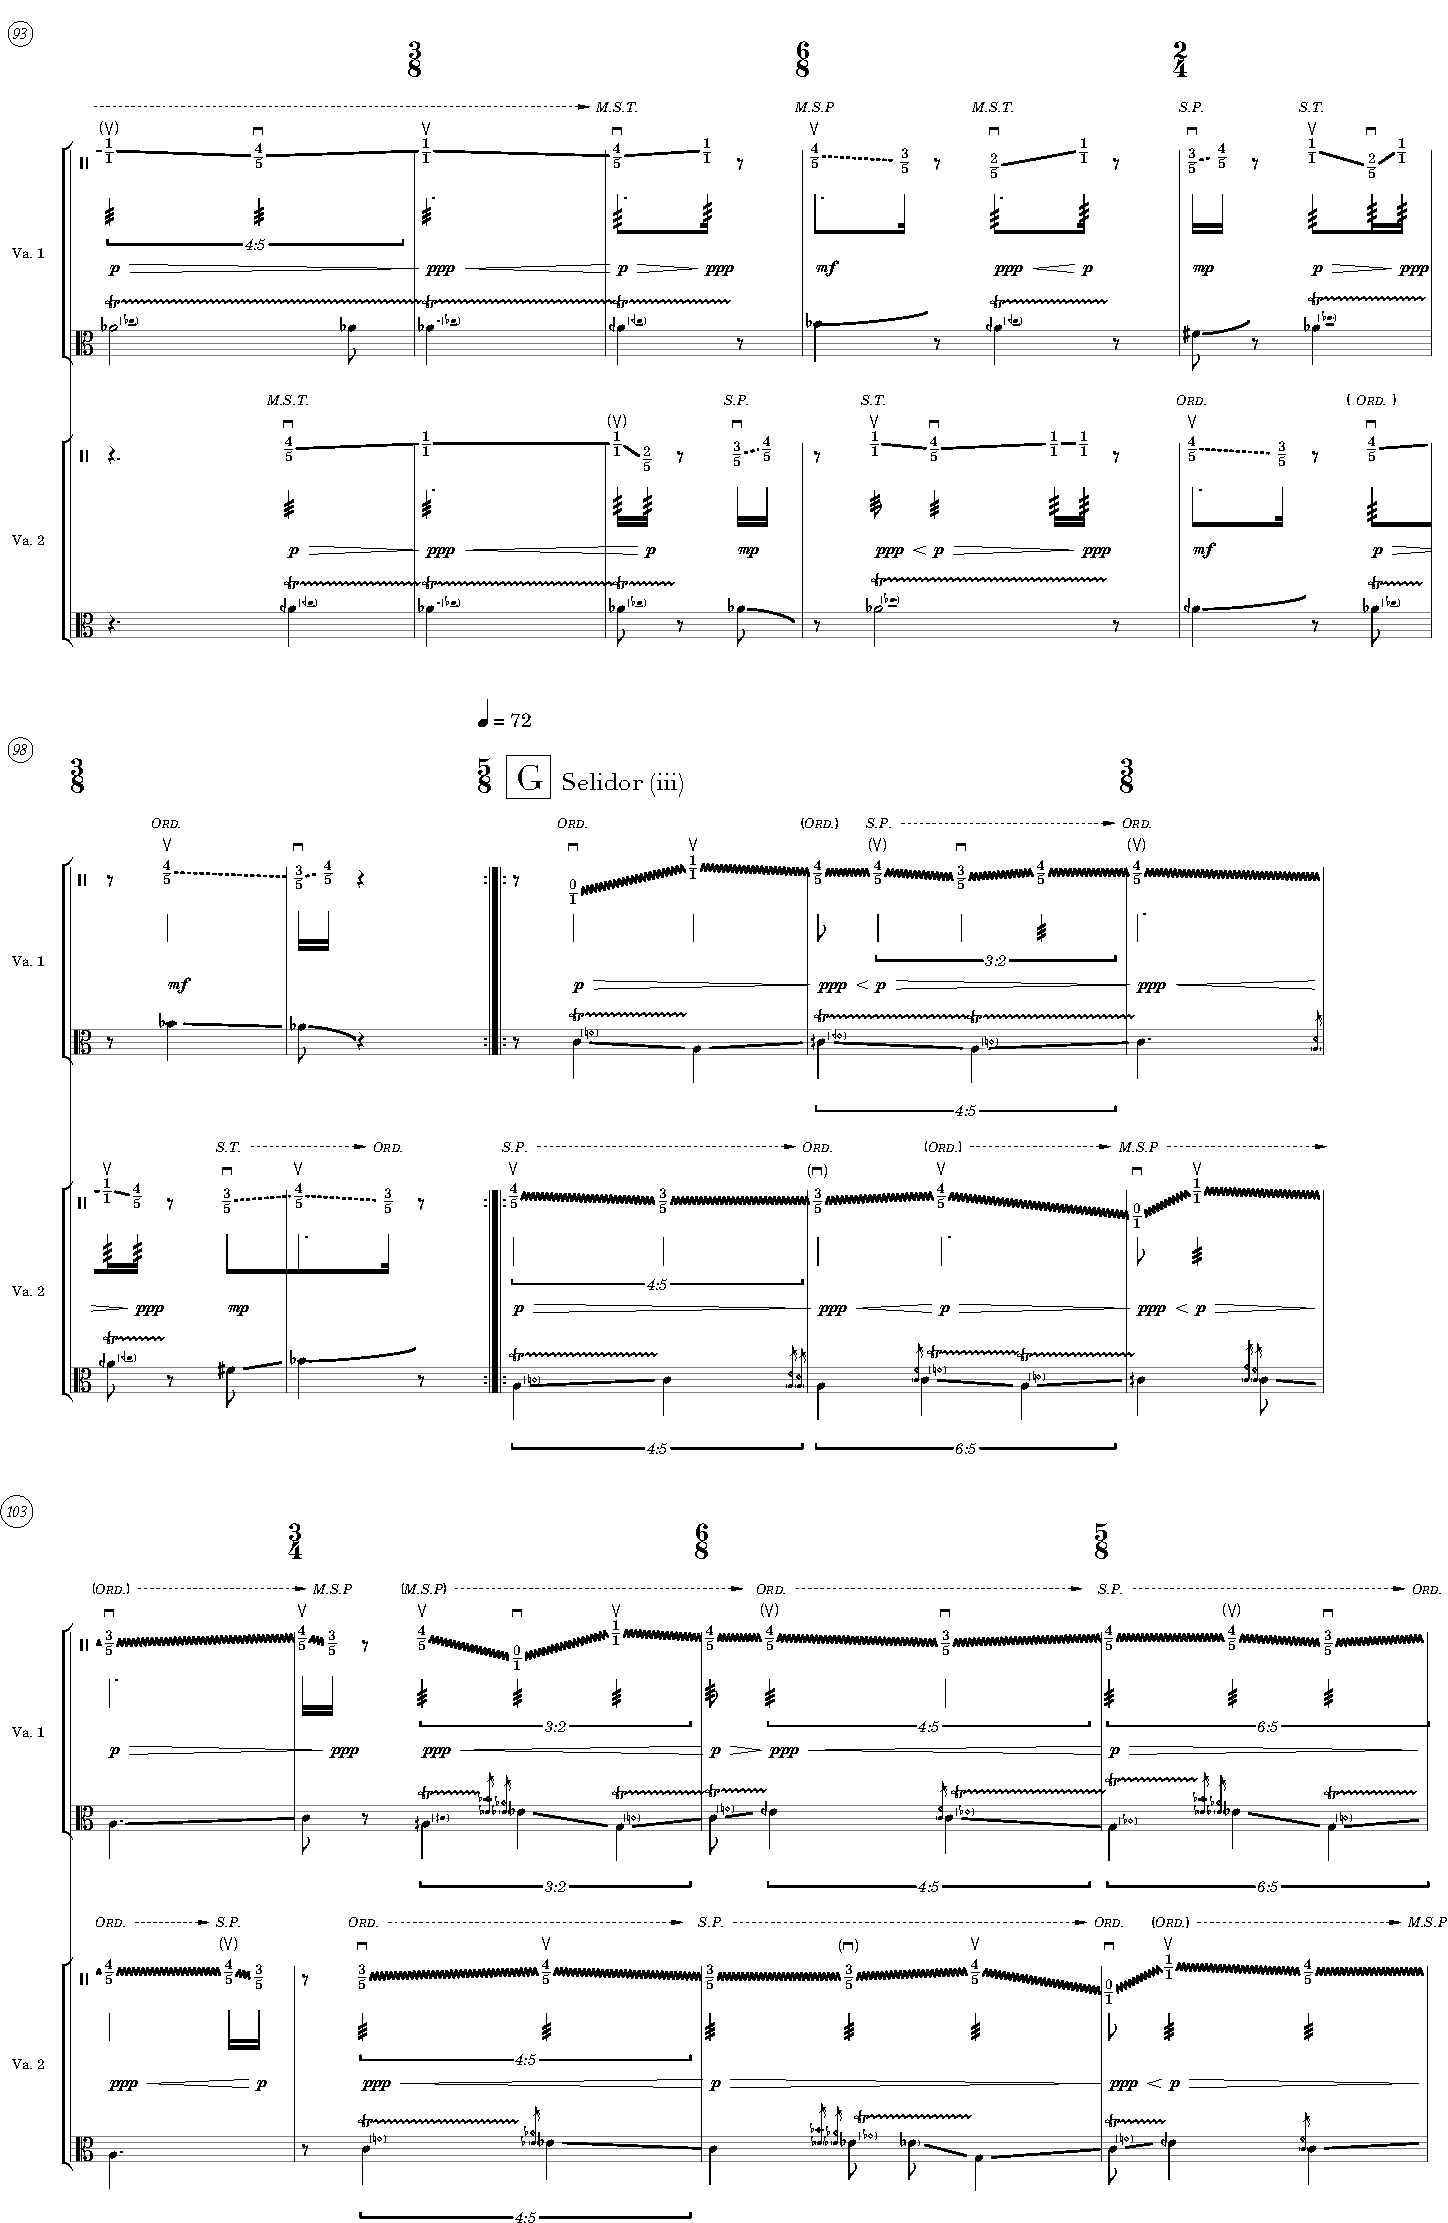
\includegraphics[height=.8\paperheight]{assets/armilla-page-8.pdf}}
    \caption{
        Page 8 from Josiah Wolf Oberholtzer's \emph{Invisible Cities (ii):
        Armilla} for two violas (2015), created with tools extending Abjad.
        Source for this score is available at
        \url{https://github.com/josiah-wolf-oberholtzer/armilla}. }
\end{figure*}

\section{Project testing and maintenance} \label{sec:development}

Abjad has benefited enormously from programming best practices developed by the
open-source community. As described previously, the extension of an existing
language informs the project as a first principle. The following other development practices
from the open-source community have also positively impacted the project and
might be helpful in the development of other music software systems.

The music software systems literature investigated in preparing this report
remains overwhelmingly silent on questions of software testing. None of the
sources cited in this article reference software test methodologies. The same
appears to be true for the larger list of sources included in
\cite{trevino2013compositional}.\footnote{Chris Ariza's work developing
AthenaCL \cite{Ariza2005} and the development of Music21 \cite{Ariza2010} led
by Michael Cuthbert are important exceptions. Both projects are implemented in
Python and both projects feature approaches to testing aligned to those
outlined above.} Why should this be the case? One possibility is that authors
of music software systems have, in fact, availed themselves of important
improvements in software test methods developed over the previous decades but
have, for whatever reasons, remained quiet on the matter in the publication
record. Perhaps the culture of software best practices now widely followed in
the open-source community simply has not yet arrived in the field of music
software systems development (and especially in the development of music
software systems designed for noncommercial applications).

The use of automated regression testing in Abjad's development makes apparent
the way in which tests encourage efficient development and robust project
continuance.\footnote{Abjad comprises an automated battery of 9,119 unit tests
and 8,528 documentation tests. Unit tests are executed by \texttt{pytest}.
Documentation tests are executed by the \texttt{doctest} module included in
Python's standard library. Parametrized tests are provided to ensure that
behaviors implemented the same way against different classes produce
corresponding output. Developers run the entire battery of tests at the start
of every development session. No new features are accepted as part of the Abjad
codebase without tests authored to document changes to the system. Continuous
integration testing is handled by Travis CI to ensure that all tests pass after every commit from every core developer and newcomer to the project alike.
For \texttt{pytest} see \textit{http://pytest.org}. For Travis CI see
\textit{https://travis-ci.org}.} The presence of automated regression tests acts as an incentive to new contributors
to the system (who can test whether proposed
changes to the system work correctly with existing features) and greatly increases the
rate at which experienced developers can refactor the system during new feature
development.
Abjad currently comprises about 178,000 lines of code, and the
Abjad repository, hosted on GitHub,\footnote{https://github.com/Abjad/abjad}
lists more than 8.7 million lines of code committed since the start of the
project. This refactor ratio of about 50:1 means that each line of code in the
Abjad codebase has been rewritten dozens of times. This freedom to refactor is
possible only because of the approach to automated regression testing Abjad has
borrowed from the larger open-source community.

Testing also benefits project continuance when the original developers of a
music software system can no longer develop the system. Automated regression
tests help make possible a changing of the guard from one set of developers to
another. Automated tests serve as a type of functional specification of how a
software system should behave after revision. While
automated tests alone will not ensure the continued development of any software
system, adherence to the testing practices of the open-source community
constitutes the most effective hedge available to music software systems
developers to fend against project abandonment in the medium and long term.

\section{Discussion \& Future work} \label{sec:discussion}

The design and development priorities for Abjad outlined here derive from the
fact that the developers of Abjad are all composers who use the system to make
their own scores. Abjad is not implemented for the type of music information
storage and retrieval functions that constitute an important part of
musicology-oriented music software systems. Nor is Abjad designed for use in
realtime contexts of performance or synthesis. Abjad is designed as a
composers' toolkit for the formalized control of music notation and for
modeling the incredible array of musical ideas that composers use notation to
explore and represent. Although Abjad embeds well in other music software
systems, future work planned for Abjad itself does not prioritize file format
conversion, audio synthesis, realtime applications or human interface
integration. Future work will instead extend Abjad for object-oriented control
over parts of the document preparation process required of complex scores with
many parts. Future work will also extend and reinforce the inventory of factory
classes and factory functions introduced in this report. We hope this will
encourage composers working with Abjad to transition from working with the
lower-level symbols of music notation to modeling higher-level ideas native to
one's own language of composition.

\begin{comment}
In architecting Abjad, we have put the
exigent needs of our own scores in dialogue with feedback from the Abjad user
community and filtered both of these through the best solutions we could find
concerning the generalization, encapsulation and testing of our code. We hope
that Abjad will give many more composers the satisfaction of modeling their own
ideas about composition in a way that encourages rigor and exploration at the
same time. We also hope Abjad will continue to encourage a rich collection of
different approaches to music-making by anchoring the work of composition in a
widely-used programming language and a detailed object-oriented model of
notation.
\end{comment}

\section{Acknowledgements} \label{sec:acknowledgements}

Our sincere thanks go out to all of Abjad's users and developers, for their
enthusiasm, support and boundless curiousity. We would also like to thank
everyone behind the LilyPond and Python projects, as well as the wider
open-source community, for fostering the tools that made Abjad possible.

\bibliography{tenor2015}
\end{document}